\chapter{Thermal history and Big Bang nucleosynthesis} \label{ch:thermal_history_and_BBN}

A complete account of the early thermal history of the universe is beyond our scope, but the basic story is this: as universe expanded and cooled, different processes dominated.  Various parts of this early history get imprinted on the in the nucleosynthesis of light atoms during the first minutes of the Big Bang and in the CMB.

The earliest history we do not understand well.  The earliest epoch for which we have some evidence is inflation, a postulated exponentially-rapid expansion that would serve to iron out spatial curvature, dilute magnetic monopoles, and generate  a nearly-scale-invariant power spectrum of initial fluctuations, both in density (scalar or curvature) and gravitational waves (tensor), by rapidly expanding quantum field fluctuations from microscopic to macroscopic to cosmological scales.  Inflation's mechanism is uncertain, but the simplest models include a scalar field that is high on a shallow potential, slowly rolling down.  Such an expansion rapidly cools the universe.

However it happens, the epoch of inflation then ends.  The field decays to standard model particles, dumping its energy density in the newborn universe and re-heating it to extremely high temperature.    The exponential expansion ends, replaced with a power law expansion of radiation domination.  This sets the initial conditions for the ``Hot Big Bang.''

We are not sure of how the next processes take place or even in what order.  Some process generates some kind or kinds of dark matter.   Some process of baryogenesis imprints an imbalance between particles and antiparticles.  Initially there are a large number of each, but as the universe cools and they annhilate, a fractional excess of $\sim 2\times 10^{-9}$ particles remains.  We know such a process must violate Baryon number conservation, C-symmetry and CP-symmetry, and be out of thermal equilibrium (the Sakharov conditions), or counter processes will simply replace the deficit of antiparticles.  Different scenarios are proposed, but we are not yet sure what happens.

\begin{figure}
  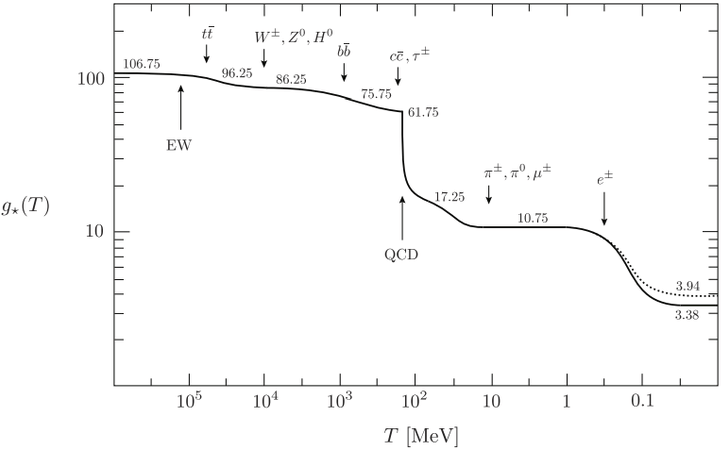
\includegraphics[width=\linewidth]{figs/CMB/gstar.png}
  \caption{Effective relativistic degrees of freedom $g_*$ in the early universe, as a function of temperature.  The solid line is the degrees of freedom for the energy density.  The dotted line is the similar expression for entropy density.  \textcolor{purple}{From Baumann, need better version.}}
\end{figure}

As the universe cools, we finally get to processes that we understand better, ones that start to be in the range of our particle accelerators.
First is the electroweak phase transition, which distiguishes photons from the $W^{\pm}$ and $Z$ bosons.  If this is a first-order phase transition, this could promote some baryogenesis (but perhaps not enough).

At this point, the temperature is still so high that all the standard model particles we know about were relativistic.  The energy density of a relativistic boson is 
\begin{equation}
 \rho_B =  g \frac{\pi}{30}  (T)^4,
\end{equation}
where $g$ is the number of (spin/polarization) states or degrees of freedom per particle. (We have $g=1$ for a massive spin-0 particle, $g=3$ for a massive spin-1 particle, or $g=2$ for a massless spin-2 boson like a photon.  Spin-1 but massless gluons have $g=16$ for 8 colors and 2 helicities.  Antiparticles double the number of states when they exist.)  This energy density comes from integrating the energy against the Bose-Einstein energy distribution function for that type of particles.  For Fermions, integrating against the Fermi-Dirac distribution yields a similar expression, but smaller by a fraction 7/8:
\begin{equation}
 \rho_F = \frac{7}{8} \times  g \frac{\pi}{30}  T^4,
\end{equation}
and again $g$ is the number of degrees of freedom. (We have $g=2$ for a spin-1/2 fermion like the electron. Spin 1/2 quarks also have 3 color states.)  When all particles are relativistic and in equilibrium with each other, at the same temperature, then the total energy density is written
\begin{equation}
 \rho =  g_*(T) \frac{\pi}{30}  T^4, \label{eq:gstar_rho}
\end{equation}
where the $g_*(T)$ is a total of the degrees of freedom available at temperature $T$.  Counting 1 for each boson and 7/8 for each fermion, we can sum up the degrees of freedom as
\begin{equation}
  g_* = \sum_{\textrm{Bosons }i} g_i + \frac{7}{8}\times \sum_{\textrm{Fermions }i} g_i \qquad \textrm{(particles relativistic)}
\end{equation}
Accounting for all known standard model particles, quarks, leptons, and force carriers, this sum yields $g_* = 106.75$.\footnote{
There is a similar expression for entropy density:\begin{equation}
 s = \frac{2\pi^2}{45} g_{*s}(T) T^3.
\end{equation}
}

The main reaction keeping particles in equilibrium is annihilation and pair-production
\begin{equation}
  p + \bar p \leftrightarrow 2 \gamma,
\end{equation}
but as the universe expands and the temperature falls ($T\propto 1/a$), particle rest masses begin to exceed the energy available in the photons.  Particles annihilate and are not replaced.  They fall out of equilibrium according to their masses, starting with the most massive, the top quark.  We can keep track of the energy density with an effective number of degrees of freedom $g_*(T)$ that keeps the form of Equation (\ref{eq:gstar_rho}) but is no longer a literal count of degrees of freedom.  (Between annihilation episodes, the $+1$ or $+7/8$ count of relativistic particles is still a pretty good approximation because relativisitic particles carry so much more energy that non-relativistic ones.)  

Reactions stop, or \textit{freeze out}\index{freeze out}, when the reaction rate falls below the Hubble rate $H(a)$.  The reaction rate
\begin{equation}
  \Gamma = n(a) \sigma(T) v(T),
\end{equation}
if the product of number density ($\propto a^{-3}$), reaction cross-section, and particle velocity ($c$ if relativistic, $\propto 1/a$ if not).  The particles become too sparse to find partners with which to react or annihilate before expansion carries them apart.  After that, there will be a negligable number of annihilation reactions, leaving some relict density, but the particles will still decay away if channels are available to them.

The top quark is the most massive particle in the standard model, so it annihlates and drops out of equilibrium first.  Next are the vector bosons of the weak force $W^\pm$ and  $Z^0$ and the Higgs boson.  These are followed by the bottom quark, charm quark, and tau lepton.  Each of these annihilations dump energy into the photon field, boosting the temperature above what it would be following the strict $1/a$ law, and the photons put it into the particles still in equilibrium.  One reason that the cold dark matter might be cold, even if it was thermally produced in equilibrium (which we don't know for sure), is that it could have been produced at such early times that subsequent annihilation of particles (standard model and unknown ones) raised the temperature of everthing else while the temperature / kinetic energy of the dark matter redshifted away to negligibility.

What follows is a dramatic change, the quantum chromodynamic (QCD) phase transition.  At this moment, free quarks in the bulk quark-gluon plasma become confined within individual baryons and mesons.  We lose all the color and spin degrees of freedom associates with those quarks and gluons as they stop participating in the equilibrium reactions.  This causes a big drop in $g_*$.  At the same time, we gain some new particles that couldn't exist before without being blasted apart by energetic photons, like protons and neutrons, which are already non-relativistic, and the pi-mesons (pions), which are still relativistic, but not for long.  These pions annihilate next, along with the muon leptons.

When the neutrinos fall out of equilibrium next, they follow a different story. Neutrinos can't directly decay to photons because they don't couple to the electromagnetic field.   At this point, the main interactions keeping the neutrinos in equlibrium are
\begin{equation}
  \nu + \bar \nu \leftrightarrow e^- + e^+   \qquad \mbox{via neutral current $Z$ boson},
\end{equation}
and
\begin{equation}
  \nu_e + e^- \leftrightarrow e^- + \nu_e   \qquad \mbox{via charged current $W$ boson, $\nu_e$ only}.
\end{equation}
Neutrinos don't decay, and leave a sizeable relict population that influences the CMB in important ways.  They still exist today, as a low-energy cosmic neutrino background, but will be extremely difficult to directly detect.

We are now about 1 second after the Big Bang.

Finally, at about 25 seconds, the electrons and positrons---the lightest charged standard model particles---fall out of equilibrium and annihilate, boosting the photon temperature in such a way to conserve entropy.  The neutrinos, having mostly decoupled by now, largely miss out on this temperate boost, and end up with a slightly lower temperature than the photons.  The electron-positron event is also the last time the photons, the light that 400k years later becomes the CMB, were in equilibrium with other particles.  The thermal equilibrium throughout the early history, with the creation and destruction of photons, establishes it as black body radiation with a Planck spectrum.  The photons continue to rapidly scatter, but these interations modify the spectrum hardly at all, and the expansion of the Universe also preserves the Planck spectrum.  {At this point there are only relativistic photons and relativistic neutrinos (at slightly lower temperature) and $g_* = 3.38$.}\footnote{Gravitons decoupled early, have very low temperature, and (probably) contribute negligibly to the radiation energy density.}

At about {200 seconds}, the temperature and density of the universe drops to the nuclear-physics energy scale, low enough to support nucleosynthesis of light elements.  Free neutrons beta decay with a half-life just over {10 minutes}.  So there is a race for successful Big Bang nucleosynthesis.  The temperature must drop enough that nascent nuclei are not immediately blasted apart by high energy photons before we run out of neutrons, which are decaying away. Deuterium, the first link in the nuclear chain, is particularly fragile, and is a bottleneck.  Eventually about 25 percent of the baryons are converted to $^4$He, with trace amounts in other nuclei up to Li and Be.  This process is complete at {about 20 minutes}.  \textcolor{purple}{We will revisit nucleosynthesis constraints on cosmology in chapter \ref{}.}
